\documentclass[hyperref={pdfpagelabels=false}]{beamer} %per eliminare un warning

\usepackage[utf8x]{inputenc}
\usepackage{default}
\usepackage[italian]{babel}
\usepackage{graphicx}
\usepackage{natbib}
\usepackage{eso-pic}


\hypersetup{pdfsubject={Synthesis of conjugated polymers and quantum dots for photovoltaics applications},pdfkeywords={polythiophene, CdSe, ligand, surface, interfaces, bulk heterojunction, phosphonic acid ligand, Sonogashira, nanocrystals, excitons, photovoltaics, solar cells, ligand exchange, pyridine, poly(3-hexylthiophene), regioregular, GRIM, asymmetric termination},pdftitle={Presentazione della tesi di laurea triennale di Ilario Gelmetti}}

\usetheme{Warsaw}        % layout complessivo. 
\useinnertheme{default} % layout interno.
\useoutertheme{default} % layout esterno.
\usecolortheme{wolverine} % schema di colori.
\usefonttheme{default}  % schema dei font.

 \AtBeginSection[]{\frame{ \tableofcontents[current,hideothersubsections]}} %indice all'inizio di ogni sezione
\let\Tiny=\tiny % per eliminare un warning
\newcommand{\diapo}[1]{\subsection{#1}\begin{frame}\frametitle{#1}}

\title{Sintesi controllata di quantum dots stabilizzati \\da polimeri coniugati funzionalizzati \\per applicazioni fotoelettroniche.}
\author{Ilario Gelmetti}
\institute{Università di Pisa}
\date{15 luglio 2010}
\logo{\includegraphics[width=0.1\paperwidth]{../tex/Immagini_Tesi/logo_unipi/unilogo_small.jpg}}

\begin{document}
\begin{frame}
  \titlepage
\end{frame}
\title{Sintesi di quantum dots stabilizzati da polimeri coniugati}


\begin{frame}
\setcounter{tocdepth}{1}
\tableofcontents
\end{frame}
\setcounter{tocdepth}{2}


\section{Funzionamento del fotovoltaico ibrido}\subsection{Ibrido: polimeri coniugati e nanoparticelle inorganiche}

%%%%%%%%%%%%%%%%%%%%%%%%%%%%%%%%%%%%%%%%%%%%%%%%%%%%%%%%%%%%%%%%%%%%%%%%%%%%%%%%%%%%%%%%%%%%%%%%%%%%%%%%%%%%%%%%%%%%%%%%%%%%%%%%%%%%

\begin{frame}
  \frametitle{Ibrido: polimeri coniugati e nanoparticelle inorganiche}

\begin{description}
 \item[Cella fotovoltaica ibrida:]{modulo fotovoltaico avente \alert{strato fotoattivo} composto sia di materiale organico che inorganico.}
\end{description}

\begin{columns}
\column{0.7\linewidth}
\begin{center}
  \begin{minipage}{6.7cm}  


 \uncover<2->{
\begin{block}{In questo lavoro di tesi:}
\begin{itemize}
 \item materiale organico: \\\alert{poli(3-esiltiofene) regioregolare \\terminato asimmetricamente},
 \item materiale inorganico: \\\alert{nanoparticelle di CdSe}.
\end{itemize}
Entrambi i materiali sono \alert{semiconduttori}.
\end{block}}\end{minipage}
\end{center}\column{0.3\linewidth}

\begin{figure}
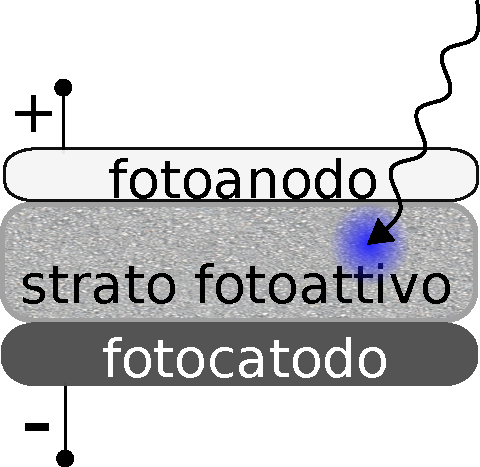
\includegraphics[width=0.9\textwidth]{Immagini_Tesi/pv-schema2.pdf}
\end{figure}
\end{columns}
\end{frame}

%%%%%%%%%%%%%%%%%%%%%%%%%%%%%%%%%%%%%%%%%%%%%%%%%%%%%%%%%%%%%%%%%%%%%%%%%%%%%%%%%%%%%%%%%%%%%%%%%%%%%%%%%%%%%%%%%%%%%%%%%%%%%%%%%%%%
{
\setbeamertemplate{navigation symbols}{}
\subsection{Assorbimento della luce e generazione di eccitoni}
\begin{frame}
\frametitle{Assorbimento della luce e generazione di eccitoni}
Un fotone assorbito dallo strato fotoattivo eccita un elettrone presente nella \alert{banda di valenza} delle \alert{nanoparticelle} o nel \alert{HOMO} del \alert{polimero}.\\


 \uncover<2->{

Se l'energia è sufficiente si formano due cariche libere, se non lo è si forma un \alert{eccitone}. Quest'ultimo è l'evento più frequente.}
\begin{figure}
\hspace{-20pt}
\centering{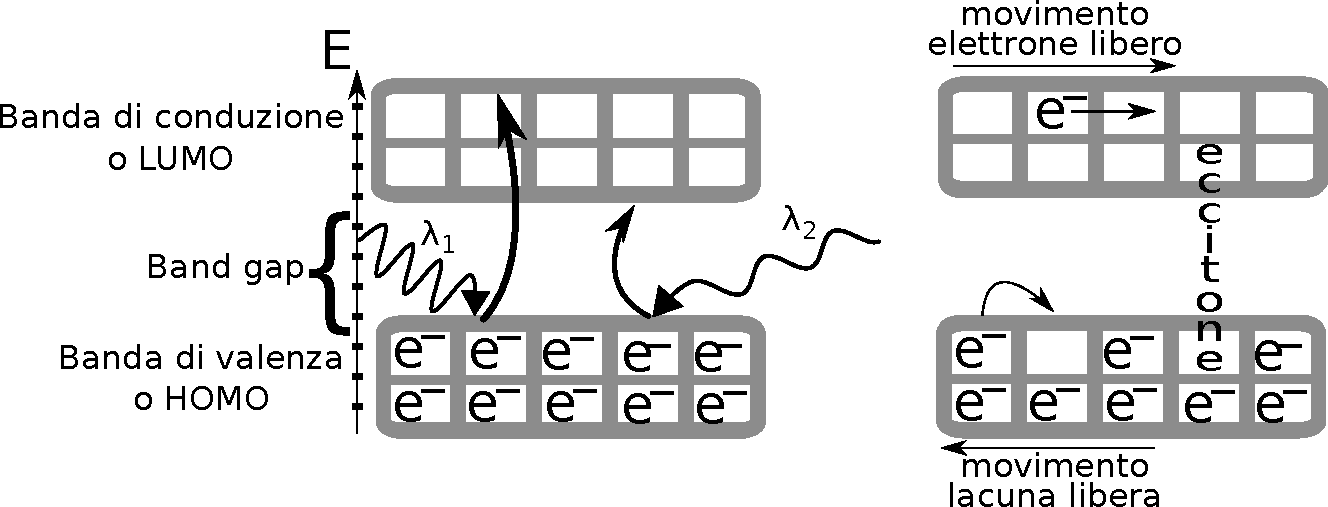
\includegraphics[width=0.9\textwidth]{Immagini_Tesi/semicond-schema2.pdf}}
\end{figure}
\end{frame}
}
%%%%%%%%%%%%%%%%%%%%%%%%%%%%%%%%%%%%%%%%%%%%%%%%%%%%%%%%%%%%%%%%%%%%%%%%%%%%%%%%%%%%%%%%%%%%%%%%%%%%%%%%%%%%%%%%%%%%%%%%%%%%%%%%%%%%

\diapo{Separazione degli eccitoni in cariche all'interfaccia}

\alert{Le coppie eccitoniche possono essere scisse in carica e lacuna per recuperarne l'energia.} 
\begin{columns}
\column{0.66\linewidth}\uncover<2->{
\begin{itemize}
 \item Sono necessari forti campi elettrici come quelli che si formano all'\alert{interfaccia} tra due semiconduttori con livelli energetici diversi.
 \item In assenza di processi di scissione si propagano in semiconduttori organici per non più di 20~nm (massimo cammino eccitonico) dopodiché decadono radiativamente.
\end{itemize}}
\column{0.34\linewidth}
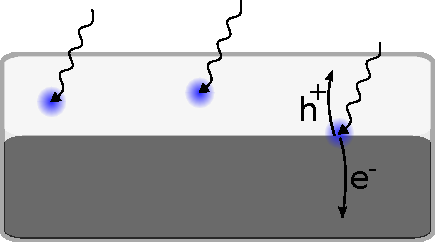
\includegraphics[width=1\textwidth]{Immagini_Tesi/bilayer-eccitoni.pdf}
\end{columns}
\end{frame}

%%%%%%%%%%%%%%%%%%%%%%%%%%%%%%%%%%%%%%%%%%%%%%%%%%%%%%%%%%%%%%%%%%%%%%%%%%%%%%%%%%%%%%%%%%%%%%%%%%%%%%%%%%%%%%%%%%%%%%%%%%%%%%%%%%%%

\subsection{Morfologia con interfaccia distribuita}
\begin{frame}
\frametitle{Morfologia con interfaccia distribuita (1)}
Una tradizionale morfologia con uno strato di polimero ed uno di nanoparticelle (\emph{bilayer}) non presenta sufficiente interfaccia.
 \begin{figure}\centering{

\includegraphics[width=.605\textwidth]{Immagini_Tesi/bulk-heterojunction-eccitoni.pdf}}\end{figure}
Una morfologia con interfaccia distribuita (\emph{bulk heterojunction}) permette di raggiungere efficienze energetiche più elevate.


\end{frame}

%%%%%%%%%%%%%%%%%%%%%%%%%%%%%%%%%%%%%%%%%%%%%%%%%%%%%%%%%%%%%%%%%%%%%%%%%%%%%%%%%%%%%%%%%%%%%%%%%%%%%%%%%%%%%%%%%%%%%%%%%%%%%%%%%%%%
\begin{frame}
\frametitle{Morfologia con interfaccia distribuita (2)}
\framesubtitle{Mantenere la morfologia \emph{bulk heterojunction} con leganti}
\begin{columns}
\column{0.68\linewidth}
\begin{block}{In questo lavoro di tesi:} Si è funzionalizzato un polimero con dei \alert{gruppi~leganti} per aumentare la disperdibilità delle nanoparticelle.\\
Tra le varie possibilità per il posizionamento dei leganti, in questa tesi è stata realizzata l'\alert{ultima in figura}.\end{block}
\column{0.3\linewidth}{\begin{figure}\centering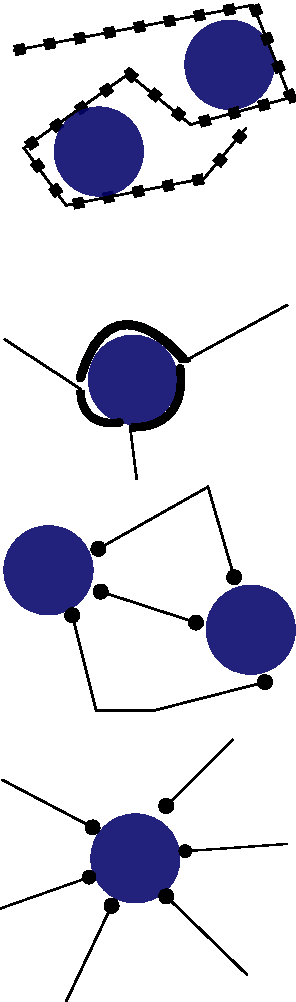
\includegraphics[width=0.5\textwidth]{Immagini_Tesi/leganti-verticale.pdf}\end{figure}}
\end{columns}
\end{frame}

\section{Caratteristiche dei materiali}
\diapo{Nanoparticelle: inorganiche o organiche?}
Le nanoparticelle vengono utilizzate come \alert{trasportatrici di elettroni}.\\
Pro e contro delle nanoparticelle inorganiche (\emph{quantum dots} semiconduttori) rispetto alle organiche (fullereni modificati o nanotubi):

\pause

 
\begin{itemize}
 \item[\checkmark] livelli energetici variabili con la dimensione,
 \item[\checkmark] coefficienti di assorbimento della luce più alti,
 \item[\checkmark] mobilità elettronica più alta,
 \item[$\times$] dimensioni maggiori dei fullereni perciò interfaccia minore,
 \item[$\times$] sono state ottenute efficienze minori a causa della \alert{aggregazione}.
\end{itemize}


\pause

 

Quest'ultimo problema si può limitare usando \\un \alert{polimero con gruppi leganti}.
\end{frame}

\diapo{Nanoparticelle inorganiche: quali? CdSe}
Molti semiconduttori inorganici si trovano in letteratura per nanoparticelle in celle ibride.
\begin{center}
  \begin{minipage}{7.5cm}   
\begin{block}{In questa tesi:} Sono state sintetizzate nanoparticelle di CdSe.\end{block}
\end{minipage}
\end{center}
\begin{itemize}
 \item efficienze energetiche più alte,
 \item anche in forme complesse.
\end{itemize}

\end{frame}

%%%%%%%%%%%%%%%%%%%%%%%%%%%%%%%%%%%%%%%%%%%%%%%%%%%%%%%%%%%%%%%%%%%%%%%%%%%%%%%%%%%%%%%%%%%%%%%%%%%%%%%%%%%%%%%%%%%%%%%%%%%%%%%%%%%%

\subsection{Polimeri coniugati: coniugazione e catene laterali}
\begin{frame}
\frametitle{Polimeri coniugati: coniugazione e catene laterali}
Il polimero coniugato assorbe la maggior parte della luce e \alert{trasporta le lacune}. \\

\pause

 

\begin{itemize}
\item Minore è la differenza HOMO - LUMO e maggiore è la porzione di spettro solare assorbito.
\item Questa differenza e la lunghezza di coniugazione dipendono dalla \alert{planarità} del polimero. 
\item Le catene laterali alifatiche aumentano la solubilità ma diminuiscono la planarità.
\end{itemize}\end{frame}

%%%%%%%%%%%%%%%%%%%%%%%%%%%%%%%%%%%%%%%%%%%%%%%%%%%%%%%%%%%%%%%%%%%%%%%%%%%%%%%%%%%%%%%%%%%%%%%%%%%%%%%%%%%%%%%%%%%%%%%%%%%%%%%%%%%%
{
\setbeamertemplate{navigation symbols}{}
\diapo{Polimeri coniugati: quale? Politiofene regioregolare}
\begin{center}
  \begin{minipage}{8.3cm}
\begin{block}{In questa tesi:}È stato sintetizzato poli(3-esiltiofene) regioregolare \\contenente un gruppo legante. \end{block}
\end{minipage}
\end{center}
Perché:
\begin{itemize}
\item livelli energetici adatti ad essere accoppiati con il CdSe, 
\item se regioregolare (vedi figura) si possono raggiungere lunghezze di coniugazione di 20 monomeri.
\end{itemize}
\begin{figure}{\centering{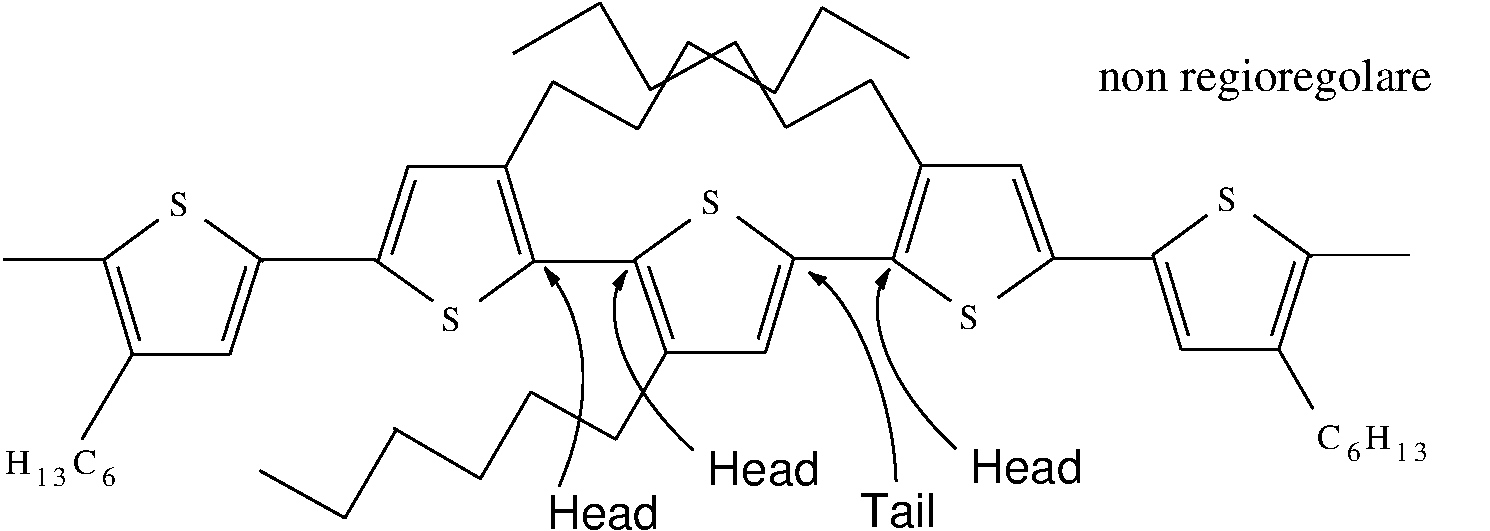
\includegraphics[width=0.67\textwidth]{Immagini_Tesi/p3ht-hhth3.pdf}}}\end{figure}
\end{frame}
}
%%%%%%%%%%%%%%%%%%%%%%%%%%%%%%%%%%%%%%%%%%%%%%%%%%%%%%%%%%%%%%%%%%%%%%%%%%%%%%%%%%%%%%%%%%%%%%%%%%%%%%%%%%%%%%%%%%%%%%%%%%%%%%%%%%%%









\section{Sistema oggetto di studio}
\subsection{Politiofene con una terminazione legante}

{
\setbeamertemplate{navigation symbols}{}

\begin{frame}
\frametitle{Politiofene con una terminazione legante}
Un possibile approccio per aumentare la dispersibilità delle NP nel polimero è \alert{rendere legante una terminazione del polimero}. \\


\pause
\begin{center}
  \begin{minipage}{8.3cm}
\begin{block}{In questo lavoro di tesi:} Si utilizzerà per la prima volta un \alert{gruppo fosfonico \\come terminazione legante}. \end{block}  
\end{minipage}
\end{center}
\begin{figure}
\centering{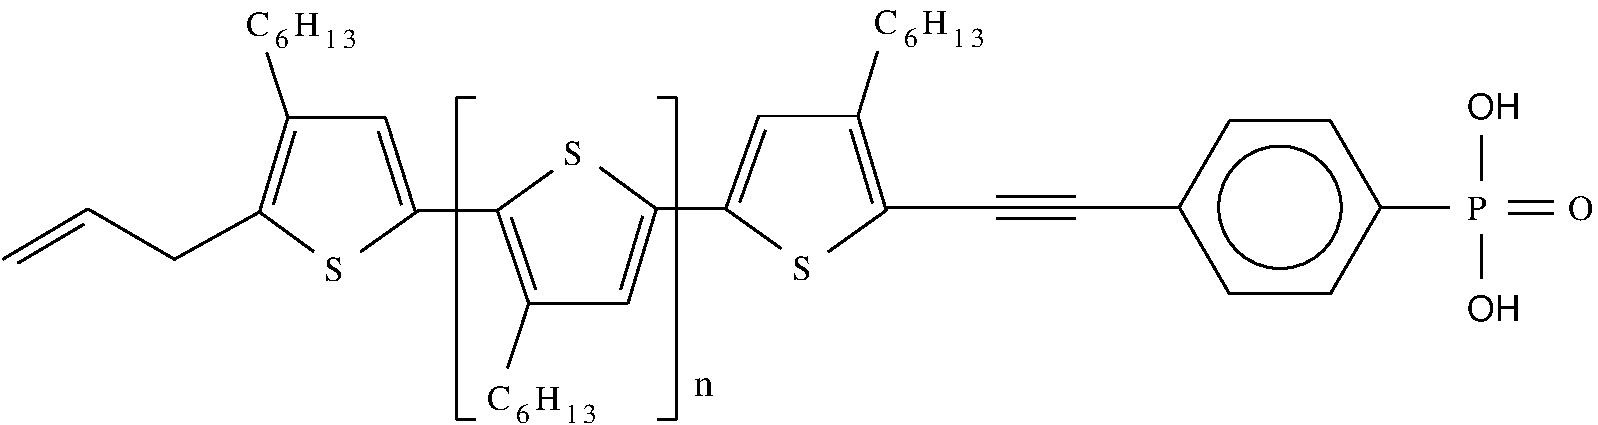
\includegraphics[width=0.7\textwidth]{Immagini_Tesi/pol-finale.pdf}}
\end{figure}
\end{frame}

}
%%%%%%%%%%%%%%%%%%%%%%%%%%%%%%%%%%%%%%%%%%%%%%%%%%%%%%%%%%%%%%%%%%%%%%%%%%%%%%%%%%%%%%%%%%%%%%%%%%%%%%%%%%%%%%%%%%%%%%%%%%%%%%%%%%%%

\diapo{Sistema oggetto di studio}
Riassumendo, la \alert{composizione} del sistema oggetto di studio è:
	\begin{itemize}
	  \item \emph{Quantum dots}: \alert{nanosfere di CdSe} $\phi = 3 - 6$~nm
	  \item Polimero: P3HT \alert{poli(3-esiltiofene) regioregolare monoterminato} con gruppo contenente un \alert{acido fosfonico}
	\end{itemize}
	Il sistema oggetto di studio dovrebbe consentire di ottenere architetture di tipo \alert{\emph{bulk heterojunction}} ovvero film sottili in cui la dispersione si avvicini ad essere bicontinua.
\end{frame}

\section{Sintesi dei materiali}
\diapo{Sintesi di nanoparticelle in micelle inverse}
Il metodo più semplice ed economico per sintetizzare nanoparticelle è la \alert{sintesi in micelle inverse}.\\
\begin{columns}
 \column{0.72\linewidth}
\uncover<2->{
\begin{itemize}
 \item Fonte di selenio: selenio in polvere.
 \item Fonte di cadmio: \alert{ossido di cadmio}\\ (più sicuro del tradizionale dimetilcadmio).
 \item \alert{Passivanti di superficie}: triottilfosfina ossido ed acido tetradecilfosfonico.
\end{itemize}}
\column{0.28\linewidth}
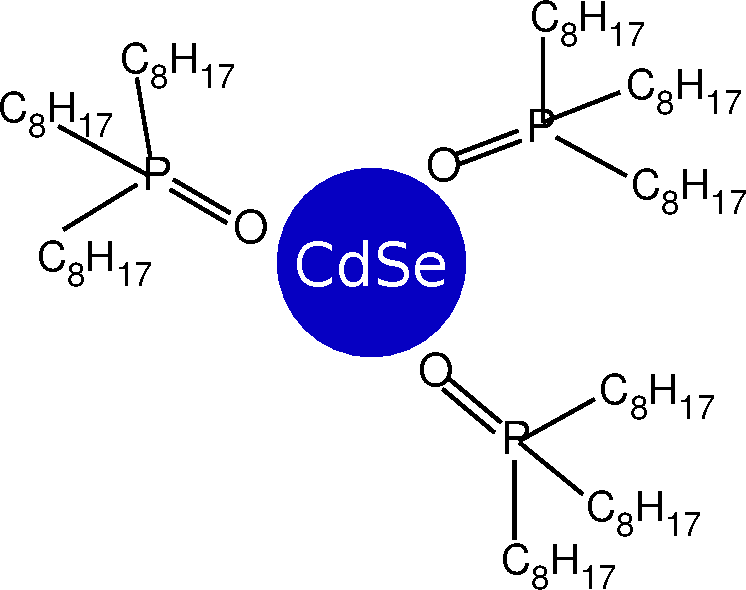
\includegraphics[width=1\textwidth]{Immagini_Tesi/CdSe-TOPO2.pdf}
\end{columns}
\end{frame}

\logo{}


\begin{frame} 
\frametitle{Caratterizzazione UV-vis e TEM}
\begin{figure}
\centering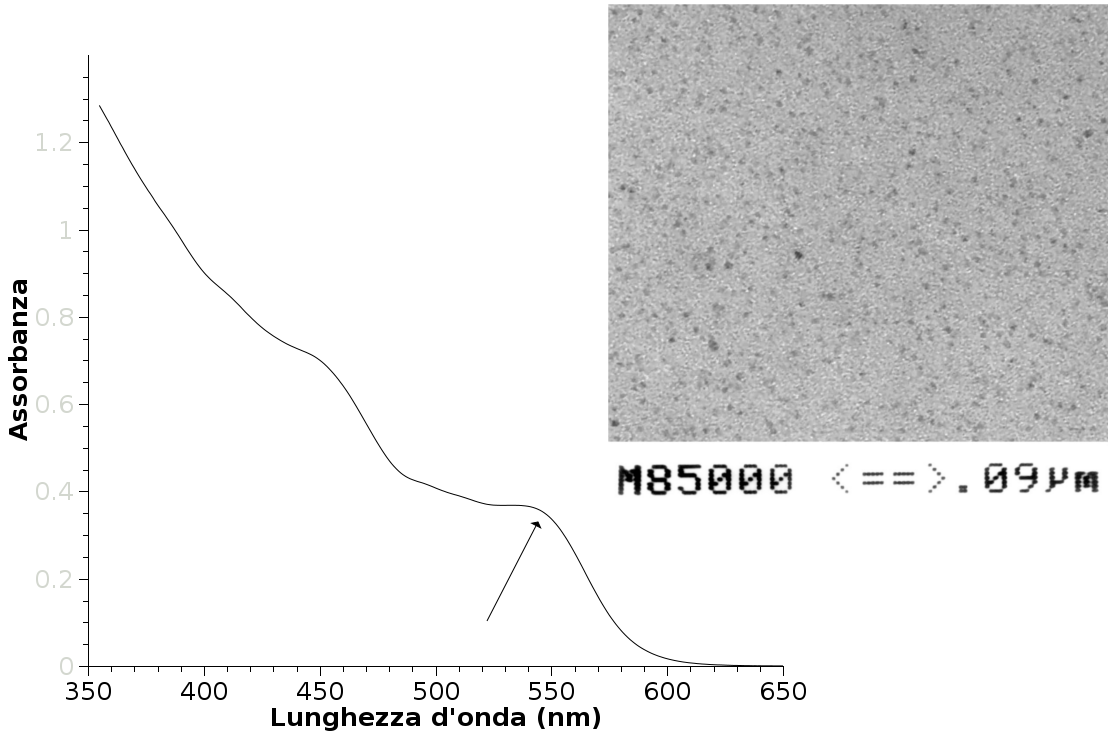
\includegraphics[width=0.9\textwidth]{Immagini_Tesi/caratterizzazione/CdSe-TOPO-UV-TEM.png}
\end{figure}
\end{frame}


%%%%%%%%%%%%%%%%%%%%%%%%%%%%%%%%%%%%%%%%%%%%%%%%%%%%%%%%%%%%%%%%%%%%%%%%%%%%%%%%%%%%%%%%%%%%%%%%%%%%%%%%%%%%%%%%%%%%%%%%%%%%%%%%%%%%


\diapo{Sintesi di poli(3-esiltiofene) regioregolare asimmetrico}

\includegraphics[width=1\textwidth]{Immagini_Tesi/pol-grim-polimerizz3.png}

\end{frame}
{
\setbeamertemplate{navigation symbols}{}
\begin{frame} 
\frametitle{Caratterizzazione $^1$H-NMR}
\vskip -10pt
\begin{figure}
\centering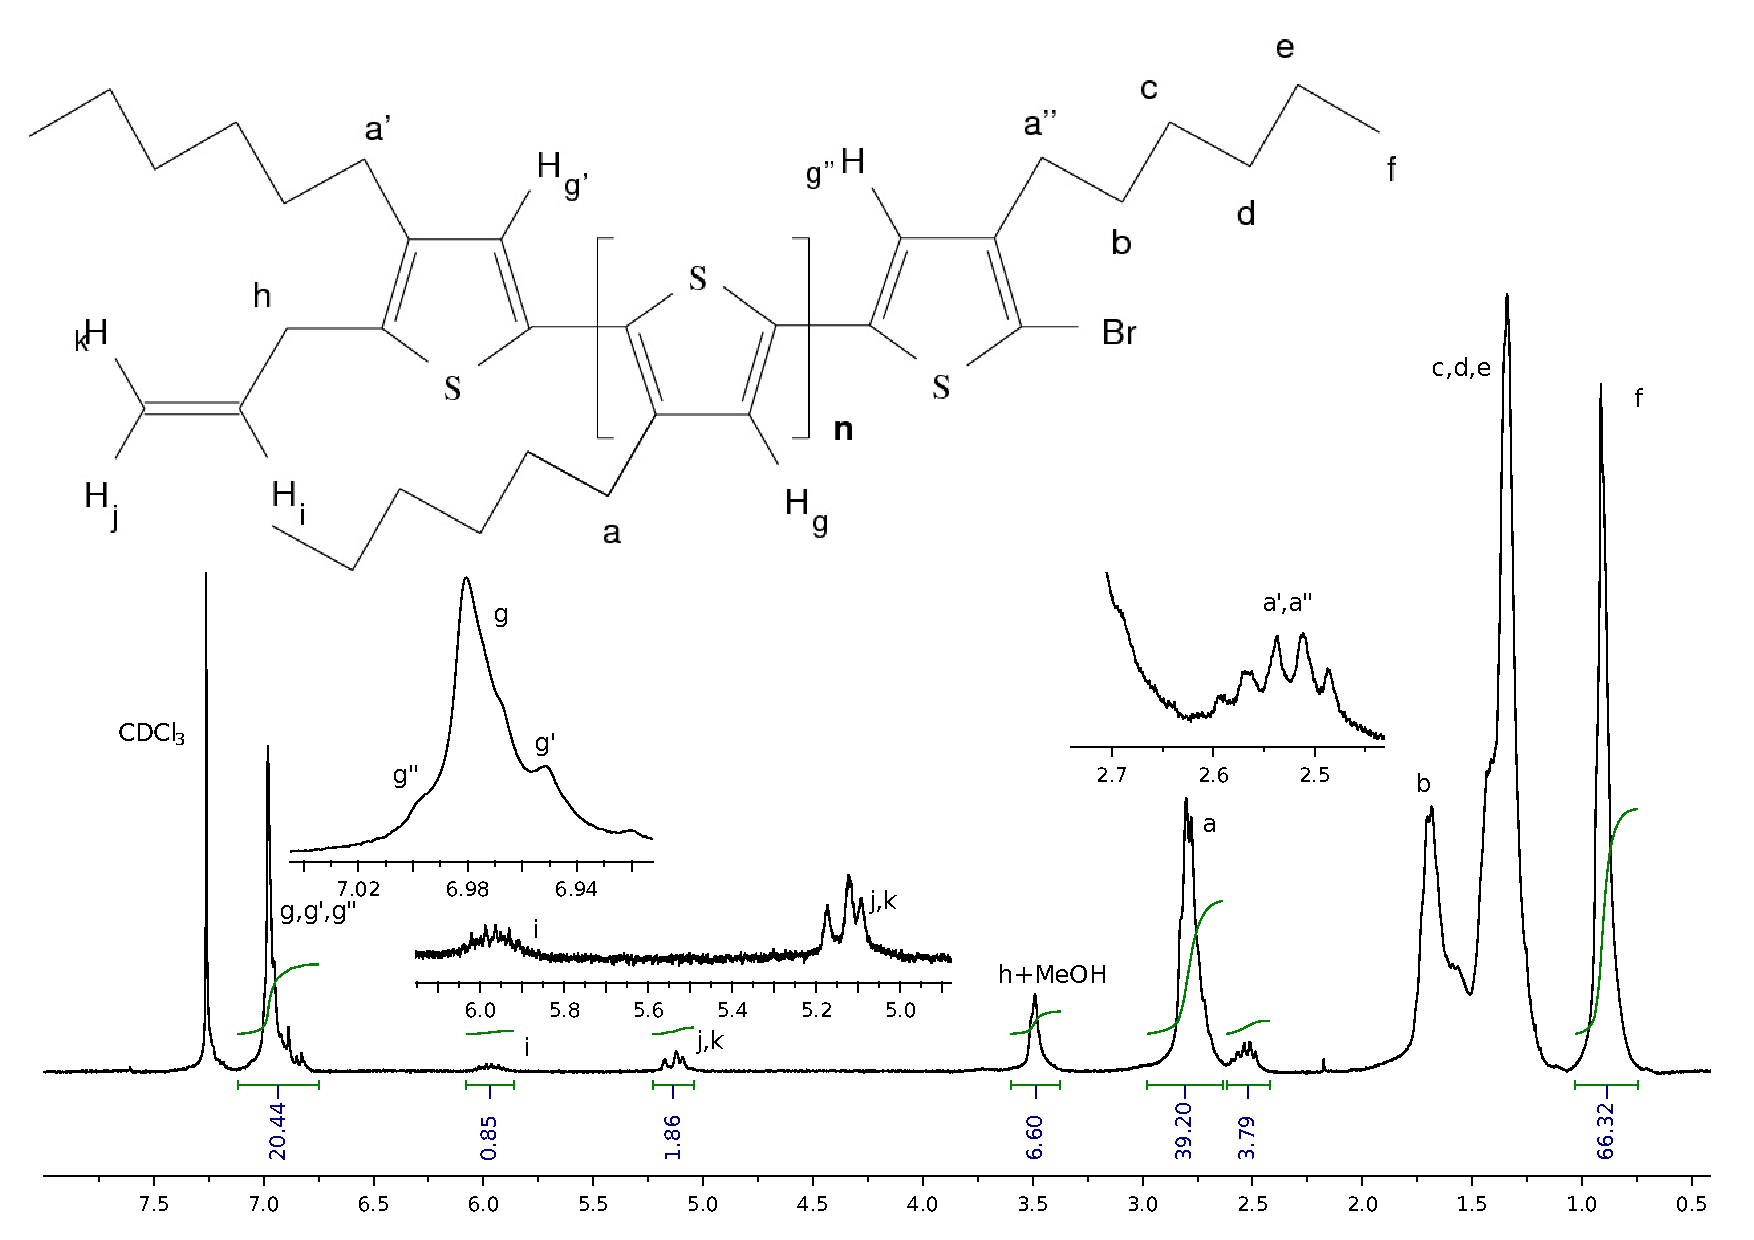
\includegraphics[width=0.98\textwidth]{Immagini_Tesi/caratterizzazione/P3HT-HNMR-3.pdf}
\end{figure}
\end{frame}

}

\logo{\includegraphics[width=0.1\paperwidth]{Immagini_Tesi/logo_unipi/unilogo_small.jpg}}

%%%%%%%%%%%%%%%%%%%%%%%%%%%%%%%%%%%%%%%%%%%%%%%%%%%%%%%%%%%%%%%%%%%%%%%%%%%%%%%%%%%%%%%%%%%%%%%%%%%%%%%%%%%%%%%%%%%%%%%%%%%%%%%%%%%%

\diapo{Attacco del legante ad una terminazione del polimero}
\begin{figure}
\centering{
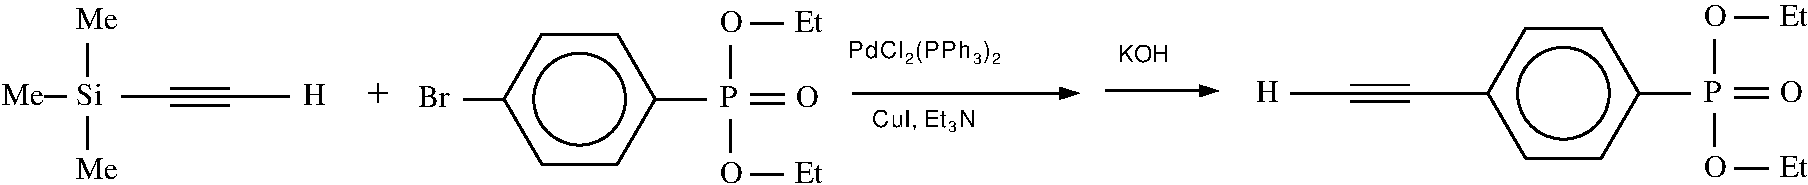
\includegraphics[width=0.8\paperwidth]{Immagini_Tesi/legante2.pdf}}\end{figure}

\begin{figure}
\centering{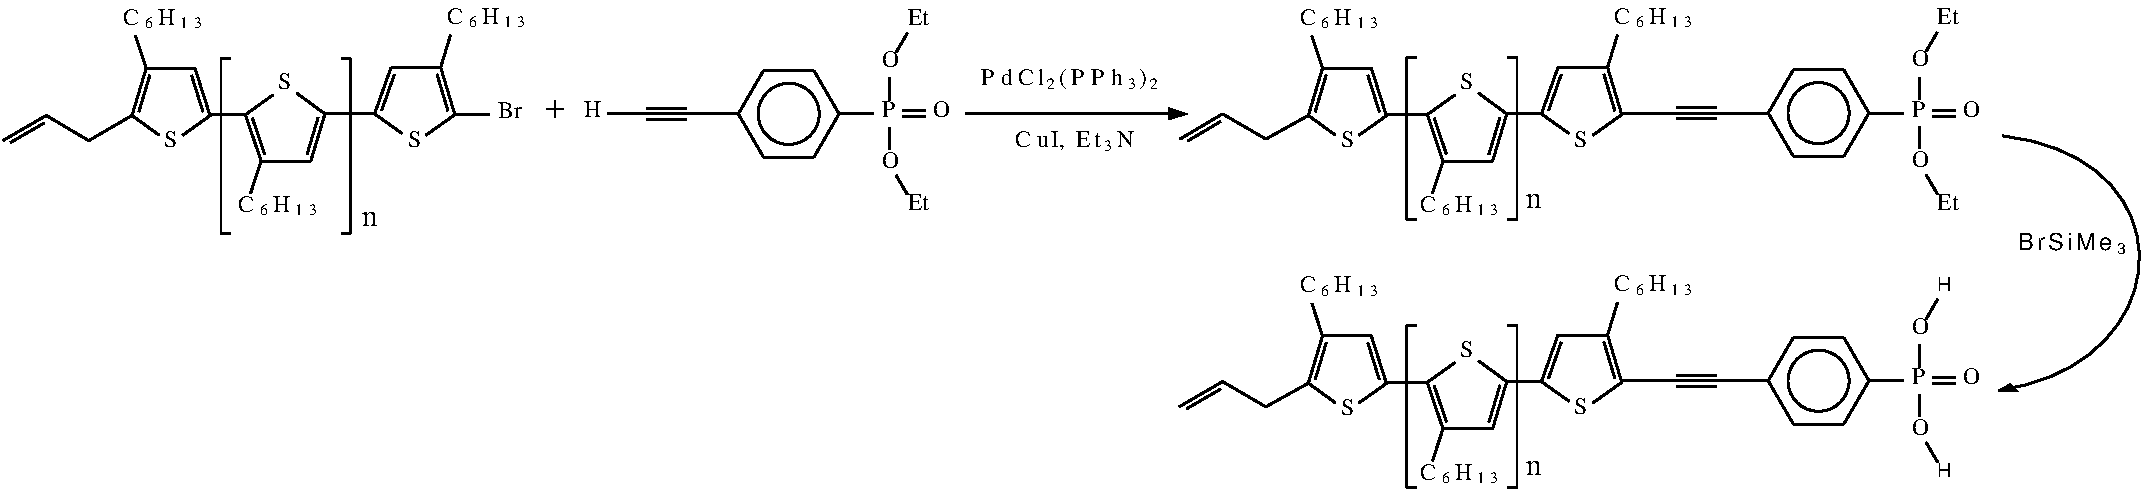
\includegraphics[width=1\textwidth]{Immagini_Tesi/p3ht-legante2.pdf}}\end{figure}
\end{frame}
{
\setbeamertemplate{navigation symbols}{}
\begin{frame} 
\frametitle{Caratterizzazione $^1$H-NMR e $^{31}$P-NMR}
\begin{figure}
\centering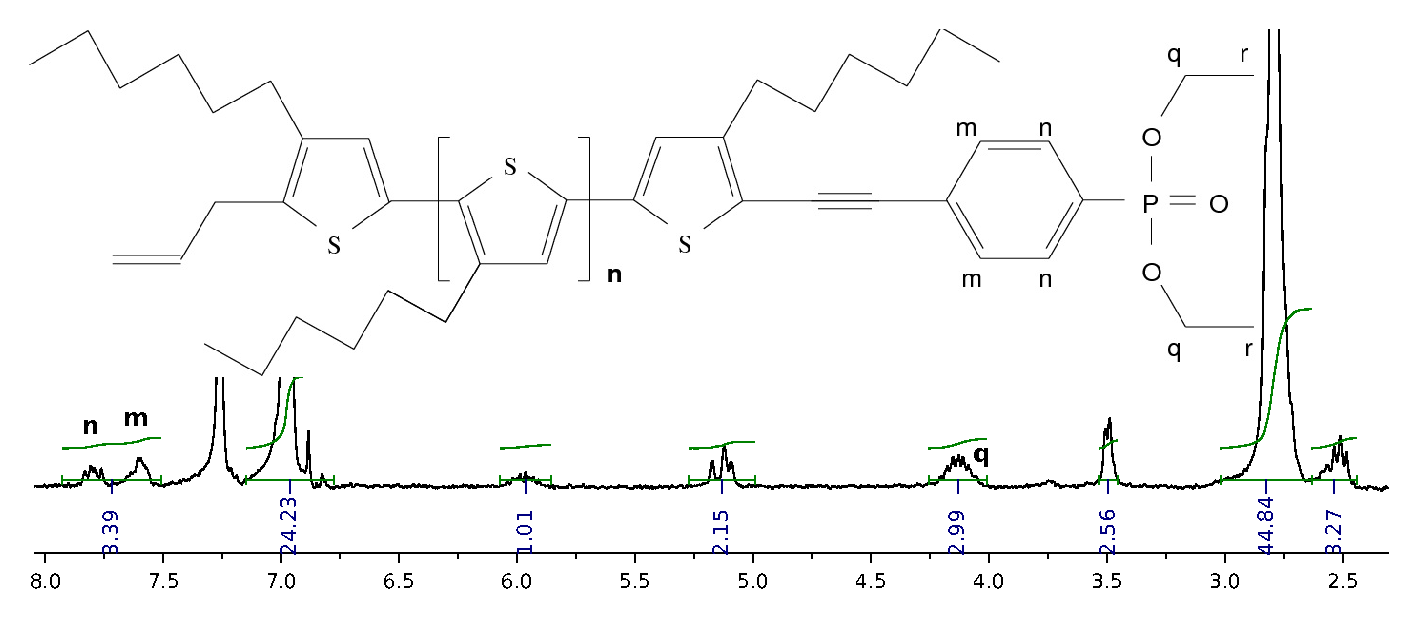
\includegraphics[width=0.85\textwidth]{Immagini_Tesi/caratterizzazione/P3HT-leg-HNMR-3.pdf}\\
\pause
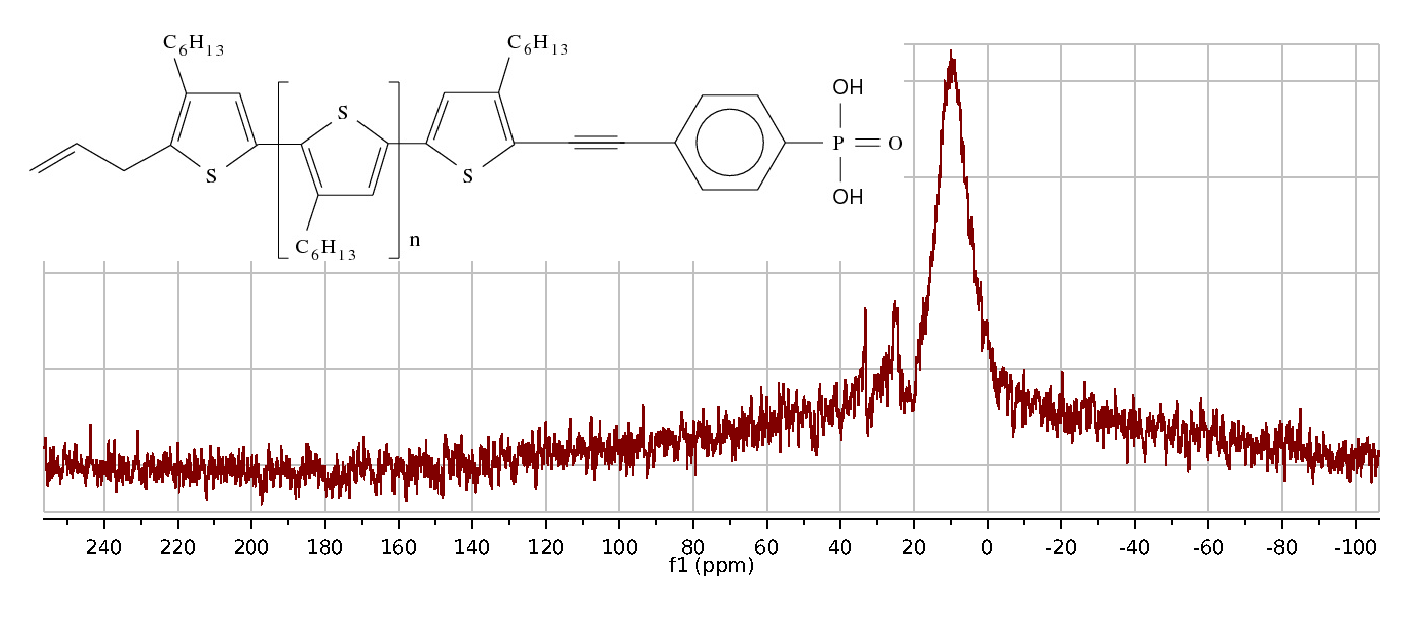
\includegraphics[width=0.7\textwidth]{Immagini_Tesi/caratterizzazione/P3HT-leg-PNMR-2.pdf}\end{figure}


\end{frame}
}
%%%%%%%%%%%%%%%%%%%%%%%%%%%%%%%%%%%%%%%%%%%%%%%%%%%%%%%%%%%%%%%%%%%%%%%%%%%%%%%%%%%%%%%%%%%%%%%%%%%%%%%%%%%%%%%%%%%%%%%%%%%%%%%%%%%%

\diapo{Scambio di leganti sulla superficie delle nanoparticelle}
\begin{figure}
	\centering{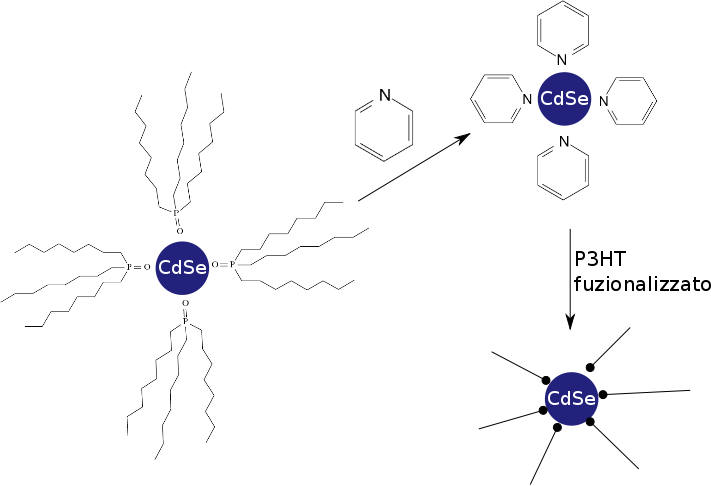
\includegraphics[width=0.8\textwidth]{Immagini_Tesi/scambio-leganti.png}}
      \end{figure}
\end{frame}
\begin{frame} 
\frametitle{Caratterizzazione UV-vis e TEM}
\begin{figure}
\centering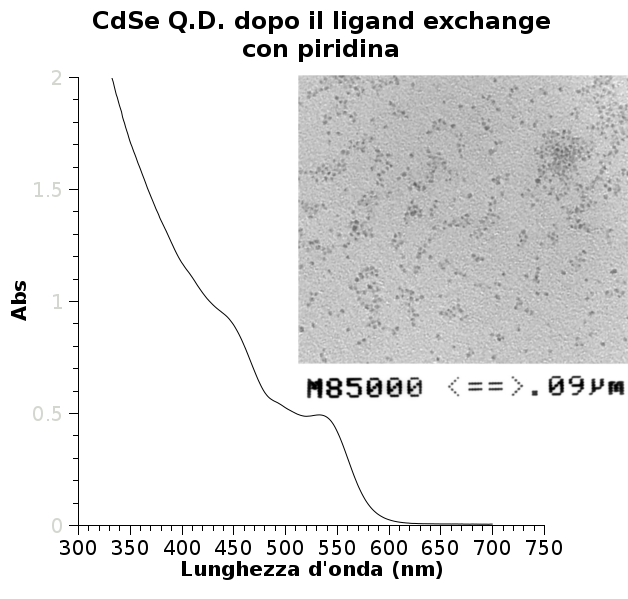
\includegraphics[width=0.5\textwidth]{Immagini_Tesi/caratterizzazione/CdSe-pyr-UV-TEM.png}\pause
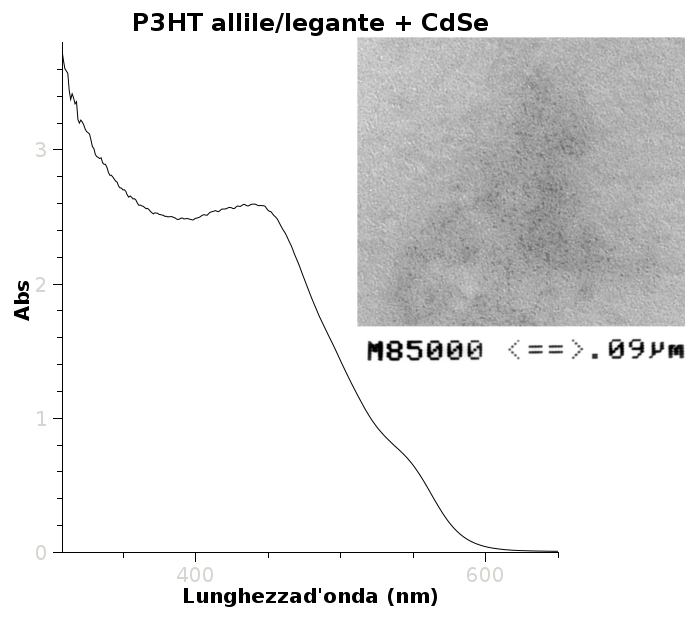
\includegraphics[width=0.5\textwidth]{Immagini_Tesi/caratterizzazione/CdSe-P3HT-UV-TEM.png}\end{figure}


\end{frame}




\section{}
\begin{frame}
\frametitle{Conclusioni}
\begin{itemize}
 \item È stato sintetizzato poli(3-esiltiofene) regioregolare monoterminato con un acido fosfonico.
 \item Il polimero sintetizzato è stato utilizzato per uno scambio di leganti su nanoparticelle sferiche di CdSe.
\end{itemize}
Il materiale sintetizzato potrebbe essere impiegato per la preparazione di strati attivi per applicazioni fotovoltaiche.
\pause
\begin{center}\line(1,0){250}\\\vskip 20pt
{\LARGE Fine.}\\ \vskip 10pt
\LaTeX ~ {\rm BEAMER} 
\includegraphics[scale=0.17]{Immagini_Tesi/debian.png}
\end{center}



\end{frame}



\end{document}
